% $Header: /data/cvsroot/Courses/OnlineLearning/talks/talk1/talk1.tex,v 1.5 2006/01/11 03:23:33 yfreund Exp $

\documentclass{beamer}
%\documentclass[handout]{beamer}
% This file is a solution template for:

% - Giving a talk on some subject.
% - The talk is between 15min and 45min long.
% - Style is ornate.

% Copyright 2004 by Till Tantau <tantau@users.sourceforge.net>.
%
% In principle, this file can be redistributed and/or modified under
% the terms of the GNU Public License, version 2.
%
% However, this file is supposed to be a template to be modified
% for your own needs. For this reason, if you use this file as a
% template and not specifically distribute it as part of a another
% package/program, I grant the extra permission to freely copy and
% modify this file as you see fit and even to delete this copyright
% notice. 


\mode<presentation>
{
  \usetheme{Montpellier}

  %\setbeamercovered{transparent}
  % or whatever (possibly just delete it)
}

\usepackage{xmpmulti} % package that defines \multiinclude

\usepackage[english]{babel}

\usepackage[latin1]{inputenc}

\usepackage{times}
\usepackage[T1]{fontenc}
% Or whatever. Note that the encoding and the font should match. If T1
% does not look nice, try deleting the line with the fontenc.

\title[Introduction] % (optional, use only with long paper titles)
{Introduction to Online Learning Algorithms}

\author[Freund] % (optional, use only with lots of authors)
{Yoav Freund}
% - Give the names in the same order as the appear in the paper.
% - Use the \inst{?} command only if the authors have different
%   affiliation.

\institute[Universities of Somewhere and Elsewhere] % (optional, but mostly needed)

\subject{Machine Learning}
% This is only inserted into the PDF information catalog. Can be left
% out. 

\newcommand{\newmcommand}[2]{\newcommand{#1}{{\ifmmode {#2}\else\mbox{${#2}$}\fi}}}
\newcommand{\newmcommandi}[2]{\newcommand{#1}[1]{{\ifmmode {#2}\else\mbox{${#2}$}\fi}}}
\newcommand{\newmcommandii}[2]{\newcommand{#1}[2]{{\ifmmode {#2}\else\mbox{${#2}$}\fi}}}
\newcommand{\newmcommandiii}[2]{\newcommand{#1}[3]{{\ifmmode {#2}\else\mbox{${#2}$}\fi}}}

\newcommand{\algfnt}{\bf}

\newmcommand{\ouralg}{{\mbox{\algfnt Hedge}({\eta})}}

\newmcommand{\iter}{T}

\newfont{\cmmib}{cmmib10}
\newcommand{\boldell}{{\mbox{\cmmib \symbol{'140}}}}

\newmcommandi{\costvec}{{\boldell}^{#1}}
\newmcommandii{\cost}{{\ell}^{#1}_{#2}}

\newmcommandi{\rd}{\tilde{#1}}

\newmcommandi{\distvec}{{\bf p}^{#1}}
\newmcommandi{\rddistvec}{\rd{\bf p}^{#1}}
\newmcommandii{\dist}{{p}^{#1}_{#2}}
\newmcommandii{\rddist}{\rd{p}^{#1}_{#2}}

\newmcommandi{\bdistvec}{{\bf q}^{#1}}
\newmcommandii{\bdist}{{q}^{#1}_{#2}}

\newmcommandi{\wtvec}{{\bf w}^{#1}}
\newmcommandi{\rdwtvec}{\rd{\bf w}^{#1}}
\newmcommandii{\wt}{{w}^{#1}_{#2}}
\newmcommandii{\rdwt}{\rd{w}^{#1}_{#2}}

\newcommand{\w}[1]{\makebox[12pt]{{#1}}}
\newcommand{\Rps}{\mbox{\tt R}}
\newcommand{\rPs}{\mbox{\tt P}}
\newcommand{\rpS}{\mbox{\tt S}}
\newcommand{\rpstie}{\w{$\frac{1}{2}$}}
\newcommand{\rpswin}{\w{$0$}}
\newcommand{\rpsloss}{\w{$1$}}

\newmcommand{\decspace}{\Delta}
\newmcommand{\decsym}{\delta}
\newmcommandi{\dec}{\decsym^{#1}}
\newmcommand{\decdistsym}{\cal D}
\newmcommandi{\decdist}{{\decdistsym}^{#1}}

\newmcommand{\simpdistspace}{{\bf \cal S}}
\newmcommand{\domset}{{\rm dom}(\decdistsym)}

\newmcommand{\expdistsym}{{\cal E}}
\newmcommandii{\expdist}{{\expdistsym}^{#1}_{#2}}
\newmcommand{\expdecsym}{{\varepsilon}}
\newmcommandii{\expdec}{\expdecsym^{#1}_{#2}}

\newmcommand{\outspace}{\Omega}
\newmcommand{\outsym}{\omega}
\newmcommandi{\out}{\outsym^{#1}}

%\newmcommandii{\Dkl}{D_{\mbox{kl}}\paren{#1||#2}}
\newmcommandii{\Dkl}{{\rm {KL}}\paren{{#1}\;||\;{#2}}}

\newmcommandi{\sumwts}{\sum_{i=1}^N \wt{#1}{i}}

\newmcommand{\lossalg}{L_A}
\newmcommand{\lossouralg}{{L_{\mbox{\scriptsize\algfnt Hedge}(\eta)}}}
\newmcommand{\lossS}{{L_{\mbox{\scriptsize\algfnt S}}}}
\newmcommandi{\lossi}{L_{#1}}
\newmcommandii{\lossit}{L_{#1}^{#2}}

\newmcommandi{\upbnd}{\tilde{#1}}

\newcommand{\angles}[1]{{\left\langle {#1} \right\rangle}}
\newcommand{\paren}[1]{{\left( {#1} \right)}}
\newcommand{\abs}[1]{{\left| {#1} \right|}}
\newcommand{\ceiling}[1]{{\left\lceil {#1} \right\rceil}}

\newfont{\msym}{msbm10}
\newcommand{\real}{\mbox{\msym R}}

\newmcommand{\updatefcn}{U_\eta}

%% \newtheorem{theorem}{Theorem}	
%% \newtheorem{lemma}[theorem]{Lemma}
%% \newtheorem{corollary}[theorem]{Corollary}
%% \newtheorem{definition}{Definition}

%\newcommand{\proof}{\noindent{\bf Proof:} }
%\newcommand{\example}[1]{{\em Example #1.} }
%\newcommand{\qed}{\rule{0.7em}{0.7em}}

\newcommand{\WeakAlg}{\mbox{\algfnt WeakLearn}}
\newcommand{\Boost}{\mbox{\algfnt AdaBoost}}
\newcommand{\EX}{\mbox{\bf EX}}
\newmcommand{\hf}{h_{{f}}}
\newmcommand{\rdhf}{\rd{h}_{{f}}}
\newmcommand{\hfT}{h^T_{{f}}}
\newmcommand{\ranh}{{b}}

\newmcommand{\conclass}{{\cal C}}

\newmcommand{\badvec}{{\bf b}}
\newmcommandi{\bad}{{b}_{#1}}

%%%%%%%% New commands defined for the game-playing paper

\newmcommand{\hedge}{\algfnt Hedge}
\newmcommand{\play}{\algfnt Play}
\newmcommandi{\Glossvec}{{\bg y}^{#1}}
\newmcommandii{\Gloss}{{y}^{#1}_{#2}}
%\newmcommandi{\action}{{I}_{#1}}
\newmcommandi{\Gdistvec}{{\bf \tilde{p}}^{#1}}
\newmcommandii{\Gdist}{{\teilde{p}}^{#1}_{#2}}

%%%%%%%%%%%%%%%%%%%%%%%%%%%%%%%%%%%%%%%%%%%%%%%%%%%%%
\newmcommand{\Idistvec}{{D}}
\newmcommandi{\Idist}{\Idistvec({#1})}
\newmcommand{\Idistt}{\Idistvec_t}

\newmcommand{\Xdist}{{\cal P}}
\newmcommand{\emp}{\hat{\epsilon}}

\newmcommand{\classpc}{Y}
\newmcommand{\numclass}{k}
\newmcommandii{\prob}{\mbox{\rm Pr}_{#1}\left[{#2}\right]}
\newmcommandii{\exval}{\mbox{\rm E}_{#1}\left[{#2}\right]}

\newmcommand{\lab}{y}
\newmcommand{\ploss}{\mbox{ploss}}
\newmcommandii{\avploss}{\ploss_{#1}({#2})}
\newcommand{\sfrac}[2]{\mbox{$\frac{#1}{#2}$}}

\newcommand{\mboosta}{\mbox{\algfnt AdaBoost.M1}}
\newcommand{\mboostb}{\mbox{\algfnt AdaBoost.M2}}
\newcommand{\mboostr}{\mbox{\algfnt AdaBoost.R}}

\newmcommand{\slos}{\mbox{ploss}}
\newmcommandiii{\sloss}{\slos_{#1}({#2},{#3})}
\newmcommandiii{\avsloss}{\slos_{{#1},{#2}}({#3})}

\newmcommandii{\vwt}{{W}^{#1}_{#2}}

\newcommand{\figline}{\rule{\textwidth}{1pt}}

%\newmcommandi{\1}{{\bf 1}({#1})}
\newmcommandi{\1}{[\![{#1}]\!]}

\newmcommand{\confcn}{\kappa}
\newmcommandi{\erint}{\abs{\int_{y_i}^{h_t(x_i)} {#1} dy}}
%\newmcommandi{\erint}{\int_{\min\{y_i,h_t(x_i)\}}^{\max\{y_i,h_t(x_i)\}}{#1}dy}


% If you have a file called "university-logo-filename.xxx", where xxx
% is a graphic format that can be processed by latex or pdflatex,
% resp., then you can add a logo as follows:

% \pgfdeclareimage[height=0.5cm]{university-logo}{university-logo-filename}
% \logo{\pgfuseimage{university-logo}}



% Delete this, if you do not want the table of contents to pop up at
% the beginning of each subsection:
%% \AtBeginSubsection[]
%% {
%%   \begin{frame}<beamer>
%%     \frametitle{Outline}
%%     \tableofcontents[currentsection,currentsubsection]
%%   \end{frame}
%% }


% If you wish to uncover everything in a step-wise fashion, uncomment
% the following command: 

\beamerdefaultoverlayspecification{<+->}

%\newcommand{\W}{\vec{W}}
%\newcommand{\V}{\vec{V}}
%\newcommand{\X}{\vec{X}}
%\newcommand{\loss}{\vec{\ell}}
%\newcommand{\HedgeLoss}{L_{\mbox{\footnotesize Hedge}}}

\begin{document}

\begin{frame}
  \titlepage
\end{frame}

\begin{frame}
  \frametitle{Outline} 
  \tableofcontents
  % You might wish to add the option [pausesections]
\end{frame}


\section{About this Course}
\begin{frame}
  \frametitle{Class web site}
  \begin{itemize}
  \item All of the class material is available from the github repository\\
    https://github.com/yoavfreund/2025-online-learning
  \item
    
\includegraphics[height=3cm]{QRcode.png}
  \end{itemize}
\end{frame}
\begin{small}
\begin{frame}
  \frametitle{What the class will cover}
  \begin{columns}
    \begin{column}[t]{3.5cm}
      \begin{itemize}
      \item Introduction (with Mean)
      \item Exponential weights algorithms
        \begin{itemize}
        \item Hedge
        \item Mixability
        \item Bregman Divergences
        \end{itemize}
      \end{itemize}
  \end{column}
  \begin{column}[t]{4.5cm}
    \begin{itemize}
    \item Online learning and Coding
      \begin{itemize}
      \item Universal Coding
      \item Continuous Experts
      \item The Context Algorithm
      \end{itemize}
    \item Multiple arm Bandit
    \item Tracking
      \begin{itemize}
      \item Tracking 
      \item Tracking within a small set of experts
      \end{itemize}
    \end{itemize}
  \end{column}
  \begin{column}[t]{4cm}
    \begin{itemize}
    \item Online learning and game theory
      \begin{itemize}
      \item Reepeated Matrix Games
      \item Internal regret.
      \item Drifting games
      \item NormalHedge
      \end{itemize}
      
    \item Online Convex Optimizatio
      \begin{itemize}
      \item Follow the regularized leader
      \item Dual Descent
      \item AdaGrad
      \end{itemize}
    \end{itemize}
  \end{column}
\end{columns}
\iffalse
    1.Introduction			15.Specialists			7.Bregman			Untitled.ipynb
10.DualDescent			2.Hedge				8.tracking			XX.OCO
11.DriftingGames		3.UniversalCodingBayes		9.trackingASmallSetOfExpert	macros.tex
12.RepeatedMatrix		4.ContinExperts			HW				plan.md
13.InternalRegret		5.ContextAlg					texput.log
14.MultipleArmBandit		6.mixable		
\fi
  \end{frame}
\end{small}

  \begin{frame}
    \frametitle{HW /  Evaluation}
    \begin{itemize}
    \item 5 HW assignments for 5*15 = 75 opints
      \item A final for 25 points.
      \end{itemize}
  \end{frame}

  % \iffalse %%%%%%%%%%%%%%%%%%%%%%%%%%%%%%%%%%%%%%%%%%%%%%%%%%%%%%%%%%%%%%%%%%
\section{Halving Algorithm}

\begin{frame} 
\frametitle{Example trace for Halving Algorithm} 

%\newcommand{\uncovered}[1]{\onslide<{#1}->\color<{#1}>{red}}

\begin{columns} 
\column[t]{3cm}
\onslide<1->\color<1>{red} 
~ \\ expert1\\ expert2\\ expert3\\ expert4 \\ expert5\\ expert6\\ expert7\\ expert8 \\ ~\\
\onslide<{2}->\color<2>{red} alg.\\
\onslide<3->\color<3>{red} outcome 
%\uncovered{3} outcome 

\column[t]{1cm}
\onslide<4->\color<4>{red} $t=1$   \\ 1 \\ 1 \\ 0  \\ 1 \\ 1 \\ 0 \\ 1  \\ 1 \\ ~ \\
\onslide<5->\color<5>{red} 1 \\
\onslide<6->\color<6>{red} 1 \\
		   			   
\column[t]{1cm}	   		   
\onslide<7->\color<7>{red} $t=2$   \\ 1 \\ 0 \\ -  \\ 0 \\ 0 \\ - \\ 1  \\ 1 \\ ~ \\
\onslide<8->\color<8>{red} 0 \\
\onslide<9->\color<9>{red} 1 \\

\column[t]{1cm}
\onslide<10->\color<10>{red} $t=3$ \\ 1 \\ - \\ -  \\ - \\ - \\ - \\ 1  \\ 1 \\ ~ \\
\onslide<11->\color<11>{red} 1 \\
\onslide<12->\color<12>{red} 1 \\
		    			     
\column[t]{1cm}	    		     
\onslide<13->\color<13>{red} $t=4$ \\ 1 \\ - \\ -  \\ - \\ - \\ - \\ 1  \\ 0 \\ ~ \\
\onslide<14->\color<14>{red} 1 \\
\onslide<15->\color<15>{red} 0 \\
		    			     
\column[t]{1cm}	    		     
\onslide<16->\color<16>{red} $t=5$ \\ - \\ - \\ -  \\ - \\ - \\ - \\ -  \\ 0 \\ ~ \\
\onslide<17->\color<17>{red} 0 \\
\onslide<18->\color<18>{red} 0 \\

\end{columns} 
\end{frame} 

\begin{frame}
\frametitle{Mistake bound for Halving algorithm}
\begin{itemize}
\item 
Each time algorithm makes a mistakes, the pool of perfect experts is halved (at least).
\item
We assume that at least one expert is perfect.
\item
Number of mistakes is at most $\log_2 N$.
\item
No stochastic assumptions whatsoever.
\item
Proof is based on combining a lower and upper bounds on the number of perfect experts.
\end{itemize}
\end{frame}

%\fi %%%%%%%%%%%%%%%%%%%%%%%%%%%%%%%%%%%%%%%%%%%%%%%%%%%%%%%%%%%%%%%%%%

\section{Perceptron}

\begin{frame}
\frametitle{The Perceptron Problem}
\begin{columns}
\begin{column}[T]{5.2cm}
\multiinclude[graphics={width=7cm},format=pdf]{perceptronAnim/Perceptron}
\end{column}

\begin{column}[T]{4cm}
\begin{itemize}
\item
$\| \V \| =1$
\item 
Example = $(\X,y)$, $y \in \{-1,+1\}$.
\item
$\forall \X,\;\; \| \X \| \leq R$.
\item
$\forall (\X,y),$\\$y(\X \cdot \V) \geq g$
\end{itemize}
\end{column}
\end{columns}

\end{frame}

\begin{frame}
\frametitle{The Perceptron learning algorithm}
\begin{itemize}
\item An online algorithm. Examples presented one by one.
\item start with $\W_0 = \vec{0}$.
\item If mistake: $(\W_i \cdot \X_i) y_i \leq  0$
\begin{itemize}
\item Update $\W_{i+1} = \W_i + y_i X_i$.
\end{itemize}
\end{itemize}
\end{frame}

\begin{frame}
\frametitle{Example trace for the perceptron algorithm}
\multiinclude[graphics={height=8cm},format=pdf]{perceptronAnim/PerceptronLearning}
\end{frame}

\begin{frame}
\frametitle{Bound on number of mistakes}
\begin{itemize}
\item The number of mistakes that the perceptron algorithm can make is at most
$\left(\frac{R}{g}\right)^2$.
\item Proof by combining upper and lower bounds on $\| \W \|$.
\end{itemize}
\end{frame}

\begin{frame}
\frametitle{Pythagorian Lemma}
~\\
If $(\W_i \cdot X_i) y <0$ then\\
\pause
\[
\| \W_{i+1} \|^2 = \|\W_i + y_i \X_i\|^2 \leq \|\W_i\|^2 + \|\X_i\|^2 
\]
\pause
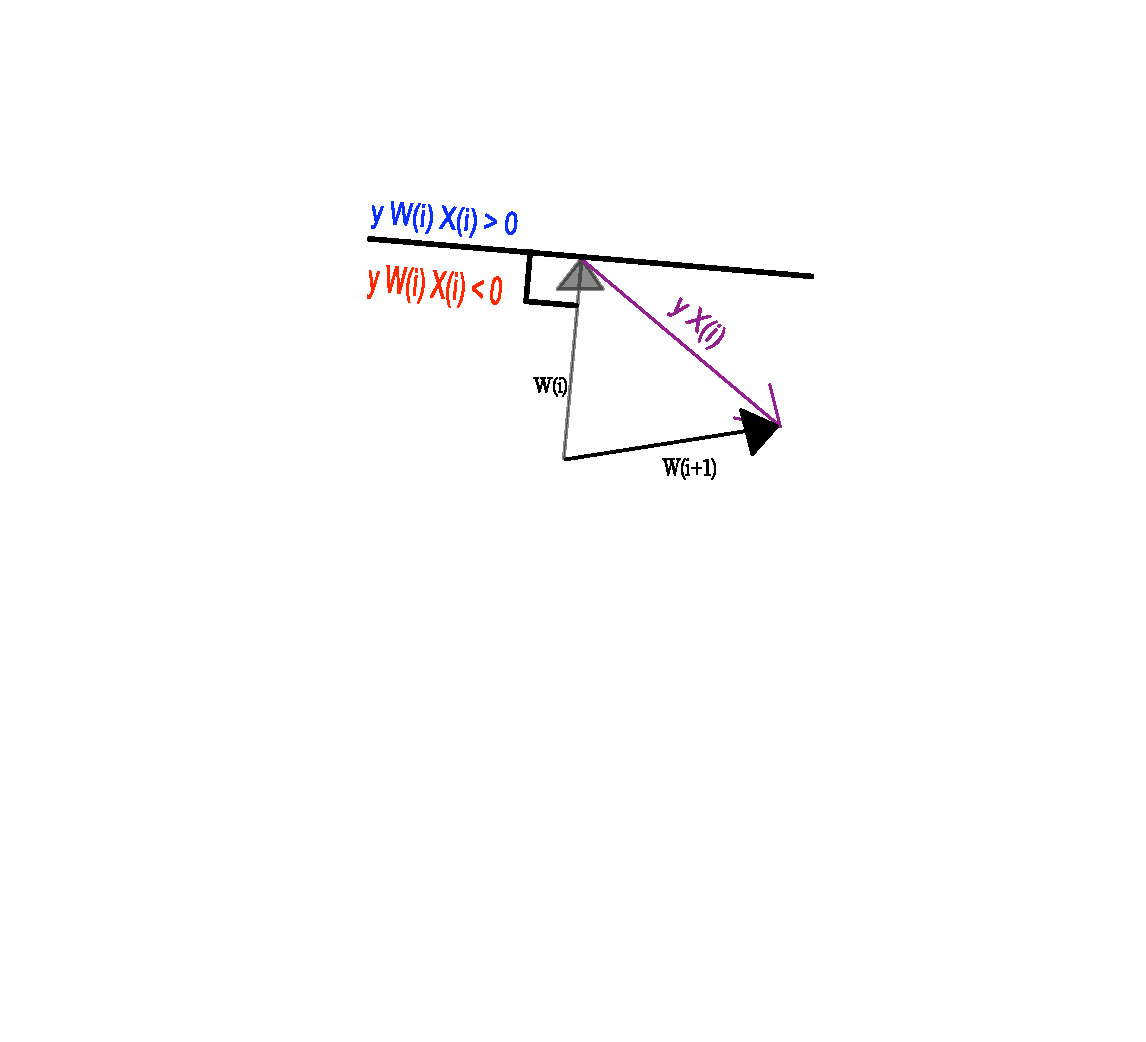
\includegraphics[height=10cm]{PerceptronAnim/PerceptronError.pdf}
\end{frame}

\begin{frame}
\frametitle{Upper bound on $\| \W_i \|$}
\pause
Proof by induction
\begin{itemize}
\item Claim: $ \| \W_{i} \|^2 \leq i R^2 $
\item Base: $i=0$, $\|\W_0\|^2 = 0$
\item Induction step (assume for $i$ and prove for $i+1$):\\
$ \| \W_{i+1} \|^2 \leq \|\W_i\|^2 + \|\X_i\|^2 $ \\
$\leq \|\W_i\|^2 + R^2 \leq (i+1) R^2$

\end{itemize}
\end{frame}

\begin{frame}
\frametitle{Lower bound on $\| \W_i \|$}
\pause
$\|\W_i\| \geq \W_{i} \cdot \V$ because $\| \V \|=1$.\\
\pause
Let $i$ denote the number of mistakes made so far.\\~\\
\pause
We prove a lower bound on $\W_{i} \cdot \V$ by induction over $i$
\begin{itemize}
\item Claim: $ \W_{i} \cdot \V \geq i g $
\item Base: $i=0$, $\W_0 \cdot \V = 0$
\item Induction step (assume for $i$ and prove for $i+1$):\\
$ \W_{i+1} \cdot \V  = \left( \W_i + \X_i y_i \right) \V$
\pause
$= \W_i \cdot \V + y_i \X_i \cdot \V$ \\
$\geq i g + g = (i+1) g$
\end{itemize}
\end{frame}

\begin{frame}
\frametitle{Combining the upper and lower bounds}
~\\
~\\
\pause
$$(ig)^2 \leq \|\W_i\|^2 \leq i R^2$$
\pause
Thus:
$$ i \leq \left(\frac{R}{g} \right)^2 $$
\end{frame}

\section{Estimating the mean}

\begin{frame}
\frametitle{The mean estimation game}
\begin{itemize}
\item 
An adversary choses a real number $y_t \in [0,1]$ and keeps it secret.
\item
You make a guess of the secret number $x_t$
\item
The adversary reveals the secret and you pay $(x_t-y_t)^2$ 
\end{itemize}
\begin{itemize}
\item You want to minimize $\frac{1}{T}\sum_{t=1}^T \left(x_t-y_t \right)^2$
\item Impossible without additional constraints.
\end{itemize}
\end{frame}

\begin{frame}
\frametitle{Adversary is a fixed distribution}
\begin{itemize}
\item 
Suppose that the adversary draws $y_1,y_2,\ldots,y_T$ IID from a fixed
distribution over $[0,1]$ with mean $\mu$ and std $\sigma$.
\item
Optimal prediction $x_t = \mu$ 
\item 
  $\exval{Y}{(\mu-Y)^2} = \sigma^2$
\item Online prediction: predict $x_{t+1}$ from $Y^t = \langle
  Y_1,Y_2,\ldots,Y_t \rangle$.
\item {\bf Expected regret}: compare performance of algorithm to
  
  $ \regret = \exval{Y^T}{(x_t-Y_t)^2} - \sigma^2$
\end{itemize}
\end{frame}

\begin{frame}
\frametitle{Individual sequence bounds}
\begin{itemize}
\item Make no assumption about how the sequence is generated.
\item The best constant value for $x$ in hind-sight:\\
  $$x^*_T \doteq \argmin_{x \in [0,1]} \sum_{t=1}^T (x-y_t)^2,\;\; x^*_T=\frac{1}{T}
  \sum_{t=1}^T y_t$$ 
\item Regret: the loss over and above the loss of $x^*_T$. {\bf for the
    worst-case sequence}
  $ \regret_T = \sum_{t=1}^T (x_t-y_t)^2 - \sum_{t=1}^T (x^*_T-y_t)^2
  $
\item {\bf Goal:} sublinear regret $\lim_{T \to \infty} \frac{\regret_T}{T} = 0$
\end{itemize}
\end{frame}

\begin{frame}
\frametitle{Follow the Leader}
\begin{itemize}
\item Idea: set $x_{t+1}$ to be the best constant prediction on $y_1,\ldots,y_t$
\item 
  $x_{t+1} = \argmin_{x \in [0,1]} \sum_{i=1}^t (x-y_i)^2 = x^*_t$ 
\item We will prove that the regret of this algorithm is upper bound
  by $2+2 \ln T$
\end{itemize}
\end{frame}
\iffalse
\begin{frame}
\frametitle{A more general setup}
\begin{itemize}
\item General euclidean space: $\vx,\vy$ are elements in $V \subset \RR^d$
\item The loss function for time step $t$ maps $\vx$ to $\RR$:\\
  $\ell_t: V \to \RR$
\item For square loss: $\elloss{\vx}{t} = (\vx -\vy_t)^2$
\item Regret relative to $\vu \in V$:
$\regret_T = \sum_{t=1}^T \elloss{\vx_t}{t} - \sum_{t=1}^T
  \elloss{\vu}{t} $
\end{itemize}
\end{frame}

\begin{frame}
\frametitle{Technical Lemma}
\begin{lemma}
  Let $\vx_t^*$ be the minimizer of $\sum_{i=1}^t \elloss{\vx}{i}$. Then
$  \sum_{t=1}^T \elloss{\vx_t^*}{t} \leq \sum_{t=1}^T \elloss{\vx_T^*}{t}$
  \end{lemma}
\end{frame}
\fi
\begin{frame}
\frametitle{Regret Bound}
\begin{theorem}
Let $y_t \in [0,1]$ for $t=1,\ldots T$ an arbitrary sequence of
numbers. Let the algorithm output be
$ x_t = x_{t-1}^* = \frac{1}{t-1} \sum_{i=1}^{t-1} y_i$, then\\
~\\
$ \regret_T = \sum_{t=1}^T (x_t-y_t)^2 - \sum_{t=1}^T (x^*_T-y_t)^2
\leq 2 \, (1 + \ln T) $
\end{theorem}
\end{frame}

\begin{frame}
%  \frametitle{Lemma 1}
  \begin{lemma}
    Let $x_1, x_2,\ldots$ be the squence of predictions produced by FTL. Then for all $u \in R$ (In particular, for $u=x^*_T$) :
    \begin{eqnarray*}
%      \regret_T(u) &=& \sum_{t=1}^T \left( (x_t-y_t)^2 - (u - y_t)^2\right)\\
 %     &\leq& \sum_{t=1}^T \left( (x_t-y_t)^2 - (x^*_{t+1}- y_t)^2\right)
	\sum_{t=1}^T \left( (x_t-y_t)^2 - (u - y_t)^2\right) \leq  \sum_{t=1}^T \left( (x_t-y_t)^2 - (x^*_t- y_t)^2\right)
    \end{eqnarray*}
  \end{lemma}
  {\bf Proof Sketch:}\\
  Subtract $\sum_{t=1}^T (x_t-y_t)^2$ from both sides to get an equivalent claim:
  \[
    \sum_{t=1}^T (x^*_t- y_t)^2 \leq \sum_{t=1}^T (u - y_t)^2
  \]
The inequality is proven by induction on $T$.
\end{frame}

\begin{frame}
\begin{proof}
\begin{itemize}
\item Base case ($T=1$): $(x^*_1 - y_1)^2 = (y_1 - y_1)^2 = 0 \le (u-y_1)^2$
\item Induction hypothesis: $\sum_{t=1}^{T-1}(x^*_t - y_t)^2 \leq \sum_{t=1}^{T-1} (u - y_t)^2$
\item Induction step:
    \begin{eqnarray*}
    	\sum_{t=1}^{T-1}(x^*_t - y_t)^2 \leq \sum_{t=1}^{T-1}(x^*_{T-1} - y_t)^2 \leq \sum_{t=1}^{T-1}(x^*_{T} - y_t)^2
    \end{eqnarray*}
    Adding $(x^*_T - y_T)^2$ to both sides gives: $$\sum_{t=1}^{T}(x^*_t - y_t)^2 \leq \sum_{t=1}^{T} (x^*_{T} - y_t)^2  \leq \sum_{t=1}^{T} (u - y_t)^2$$
\end{itemize}
\end{proof}
\end{frame}

%\begin{frame}
%\frametitle{Sketch of proof of theorem}
%Using the fact that FTL is $x^*_t = \frac{1}{t-1} \sum_{i=1}^{t-1} y_i$ \\
%one can show that $x_{t+1}^*-y_t = \frac{t-1}{t} (x_t^* - y_t)$\\
%and therefor that $(x_t^*-y_t)^2 - (x_{t+1}^*-y_t)^2 = \frac{1}{t} (x_t^* - y_t)^2$\\
%%and that $(x_t^*-y_t)^2 - (x_{t+1}^*-y_t)^2 \leq \frac{1}{t} (x_t^* - y_t)^2$
%From the fact that $0\leq x_t^*,y_t \leq 1$ we get that $(x_t^*-y_t)^2\leq 1$.\\
%From which we obtain $\sum_{t=1}^T ((x_t^* - y_t)^2-(x_{t+1}^* - y_t)^2) \leq
%\sum_{t=1}^{T} \frac{1}{t}$\\
%Combing the last statement with the Lemma concludes the proof of the theorem.
%
%\end{frame}


\begin{frame}
\frametitle{Proof of the theorem}
First, note that in FTL we have:
\[
x_t = x^*_{t-1} = \frac{1}{t-1} \sum_{i=1}^{t-1} y_i = \frac{t}{t-1} \cdot \left(\frac{1}{t} \sum_{i=1}^{t} y_i - \frac{y_t}{t}\right) = \frac{t}{t-1} \cdot \left(x^*_t - \frac{y_t}{t}\right)
\]
Subtracting \(x^*_t\) from both sides, we get \(x_t - x^*_t = \frac{x^*_t - y_t}{t-1}\). Then:
    \begin{eqnarray*}
    	&\regret_T &= \sum_{t=1}^T (x_t-y_t)^2 - \sum_{t=1}^T (x^*_T-y_t)^2\\
	& &\le \sum_{t=1}^T  (x_t-y_t)^2 - (x^*_t-y_t)^2  \quad\quad (\mathrm{Lemma})\\
	& &= \sum_{t=1}^T (x_t + x^*_t - 2y_t)(x_t - x^*_t) \leq \sum_{t=1}^T \frac{2}{t-1} \leq 2\, (1 + \ln T)
     \end{eqnarray*}
\end{frame}


\end{document}

\begin{itemize}
  \item HW for next monday: prove the theorem.
\end{itemize}


%%% Local Variables:
%%% mode: latex
%%% TeX-master: t
%%% End:
